\documentclass[11pt,a4paper]{article}
\usepackage[margin=2.2cm]{geometry}
\usepackage{times}
\usepackage{booktabs}
\usepackage{pgfplots}
\pgfplotsset{compat=1.16}
\setlength{\parindent}{0pt}
\setlength{\parskip}{6pt}

\title{Virtual Switch: Lock Benchmark}
\author{Umair Abbas \quad (bsai24077)}
\date{}

\begin{document}
\maketitle
\vspace{-1.5em}

\textbf{What is measured.} \texttt{./bench} starts 1 to 12 threads that use one MAC
table at the same time. Each thread does 400{,}000 operations: 90\% lookups and
10\% updates, on 512 MACs, like a switch where most frames go to MACs it already
knows. The table is the same in every run (16 buckets, chained, same hash as the
switch); only the locking changes:

\begin{itemize}
\setlength{\itemsep}{0pt}
\item \textbf{global}: one mutex for the whole table;
\item \textbf{striped}: one mutex per bucket (what the switch uses);
\item \textbf{rwlock}: one read-write lock; lookups share it, updates take it alone.
\end{itemize}

Each number is the median of 3 runs, on a 12-core laptop, built with the course
flags (\texttt{-O0}). Throughput is million operations per second for all threads together.

\begin{center}
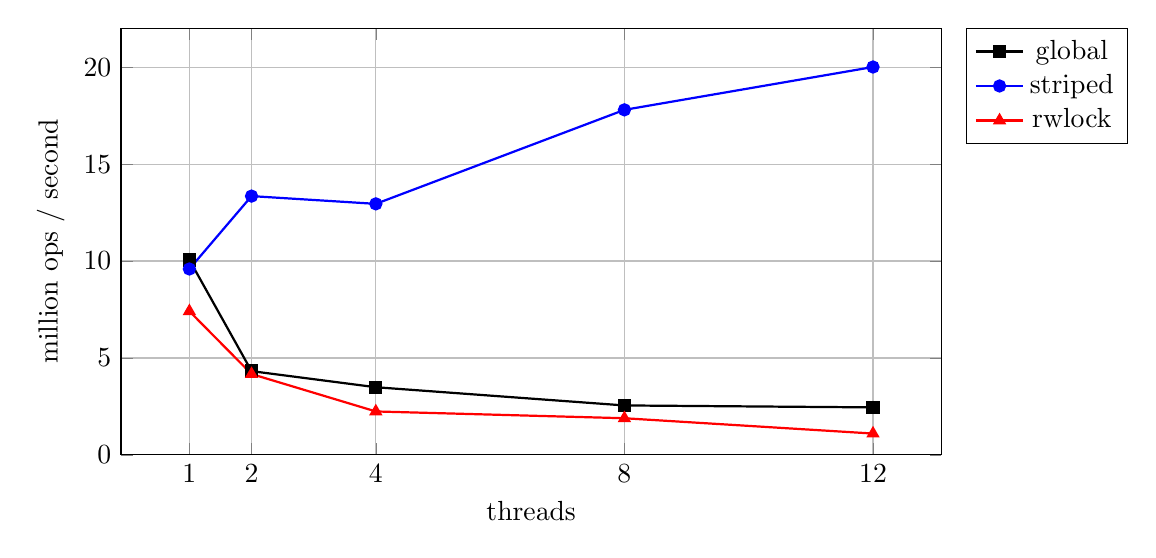
\begin{tikzpicture}
\begin{axis}[width=12cm, height=7cm, xlabel={threads}, ylabel={million ops / second},
  xtick={1,2,4,8,12}, ymin=0, legend pos=outer north east, grid=major]
\addplot[mark=square*, thick] coordinates {(1,10.06) (2,4.32) (4,3.49) (8,2.55) (12,2.45)};
\addplot[mark=*, thick, blue] coordinates {(1,9.59) (2,13.35) (4,12.95) (8,17.80) (12,20.01)};
\addplot[mark=triangle*, thick, red] coordinates {(1,7.41) (2,4.17) (4,2.24) (8,1.89) (12,1.10)};
\legend{global, striped, rwlock}
\end{axis}
\end{tikzpicture}
\end{center}

\begin{center}
\begin{tabular}{rrrr}
\toprule
threads & global & striped & rwlock \\
\midrule
1 & 10.06 & 9.59 & 7.41 \\
2 & 4.32 & 13.35 & 4.17 \\
4 & 3.49 & 12.95 & 2.24 \\
8 & 2.55 & 17.80 & 1.89 \\
12 & 2.45 & 20.01 & 1.10 \\
\bottomrule
\end{tabular}
\end{center}

\textbf{Result.} With one thread all three are about the same; the read-write lock
is a little slower because it does more work per lock. With more threads the
\textbf{global lock} gets slower, because every thread waits for the same lock and
the lock's cache line moves between cores all the time. The \textbf{read-write lock}
is the worst: lookups may share it, but every lock and unlock still writes the
reader count in one shared place, so the cores fight over it just the same, and the
10\% writers make the readers wait. \textbf{Striped locks} get faster with more
threads, because two threads only meet when they use the same one of 16 buckets.

This is why the switch uses striped locking for its MAC table.

\end{document}
